\documentclass[11pt,a4paper]{article}

\usepackage[utf8]{inputenc}
\usepackage[english]{babel}
\usepackage{graphicx}

\title{Principles of Computer System Design\\Assignment 1}
\author{Jacob Wejendorp\\Sebastian Paaske Tørholm\\Kasper Fabæch Brandt}

\begin{document}
\maketitle
\section{Exercises}
\subsection{Question 1, Fundamental abstractions}
\subsubsection{Model for implementing shared address space}
One could model an address in the shared address space as a 2-tuple of two
elements; the address or identifier of a machine, and the address on the given
machine. This is highly scalable, as each component is separated and each of
the two addresses can be interpreted independently. With suitable encoding,
no limitation is needed on the size of either the machine address or memory
address.

This model requires a naming service to determine what address each machine
has. This address could, for instance, be an IP address.

\subsubsection{Pseudocode for implementation of READ/WRITE}

\begin{verbatim}
def READ((machineaddr, dataaddr)):
    machine = connect(machineaddr)
    data = machine.read(dataaddr)
    machine.disconnect()

    return data
\end{verbatim}

\begin{verbatim}
def WRITE((machineaddr, dataaddr), data):
    machine = connect(machineaddr)
    machine.write(dataaddr, data)
    machine.disconnect()
\end{verbatim}

Here, \texttt{connect} is a function that produces a connection object to
communicate with the given machine, and said object has a \texttt{read} and
\texttt{write} method that works locally on that machine.
Pattern matching is used to extract the parts of the address from the full
address (tuple).

\subsubsection{Are READ/WRITE against memory atomic?}
On most architectures, reads and writes of a word size is atomic. Larger 
reads/writes tends to be conducted in software through smaller writes,
without explicit hardware support for atomic large transfer of data.

Most commonly, a write would be expected to be atomic by the programmer using
the service. As such, implementing atomicity would most likely be desired, since
partially written data in many contexts would be considered corrupt.

Atomicity could be achieved using one of the locking mechanisms mentioned
in the lectures. Locking could be done on a per-machine basis, or the
memory space of each machine could be split into regions, for which locks
must be held to perform operations. This could be further expanded to use
shared/exclusive locks and so on.

\subsection{Question 2, Hardware trends}

\begin{table}[h!]
    \centering

    \begin{tabular}{|r|c|c|c|}
        \hline
                        & HDD & SSD & RAM\\\hline
        Access time     & 10.000 us & ~100us & 0.1 us\\\hline % Source: slides from lecture 3, and http://en.wikipedia.org/wiki/Solid-state_drive
        Capacity (GB)   & 1000-2000 & 128-256 & 1-4 \\\hline
        Cost (kr/GB)    & 0.35 & 4.5-5.5 & 32 \\\hline
        Reliability (1-5)*& 3 & 2 & 5\\\hline % Woop
        Power consumption & $<$8w & 0.15W & ~1.65W \\\hline 
        % Datasheets: Samsung Spinpoint F1 1TB disk, Samsung 830 SSD and Samsung DDR3 ram
        % http://www.samsung.com/us/business/semiconductor/news/downloads/dsF11008.pdf
        % http://www.samsung.com/us/business/oem-solutions/pdfs/PM830_mSATA%20SSD_32_64_128_256GB_Spec_1.0.pdf
        % http://www.samsung.com/global/business/semiconductor/file/2011/product/2011/6/24/013928ds_k4b1g1646g_x16only_rev111.pdf
        
    \end{tabular}
    \caption{Rule of thumb hardware specifications.}
\end{table}
Capacity and cost pr capacity data retrieved from EDBpriser.dk, Nov 29 2012.
Ram - 1 block at a time, no sets. Power consumption data retrieved from Samsung datasheets for
Spinpoint F1 HDD, 830 SSD and DDR3 ram.

Reliability is judged on a scale from 1 to 5, where 5 is the best.
RAM is given the highest reliability, because the RAM is as reliable
as the system it is in, meaning only sudden shutdowns can cause data-loss,
which is easily handled with a UPS and emergency shutdown procedures.
SSDs are a relatively new technology, meaning that consumer SSDs often
are suffering from firmware errors. The second threat to SSDs is the limited
number of writes to a memory cell, making the lifetime expectancy comparable
to that of a mechanical harddisk.

\subsubsection{What technologies would you use for Q1?}
Main memory is used as a buffer for reads and writes. SSDs or HDDs will be used in order to gain persistence of the data.
If the average read/write size of the service is large, the gains from using SSDs will be neglible in relation to the increased cost,
making HDDs the best choice. If, however the service is a high-performance small-file storage for instance, SSDs will be favorable.


\subsection{Question 3, Performance}
\subsubsection{How does concurrency influence latency?}

The latency will be lower, if the overhead of scheduling, work partitioning and
other concurrency related overhead is less than the gain from parallelizing the
computation and vice versa. This will in practice favor larger computations and
datasets, while influencing smaller jobs negatively.

\subsubsection{What is the difference between dallying and batching?}

Batching is the act of performing several related actions simultaneously.
Dallying is the act of postponing an action, in order to later potentially batch
the action together with another related action, or maybe avoid doing it at all.

As an example, we can look at memory mapped files, where data is read from the
disk in batches (pages).
Write requests are dallied by only writing changes to ram, postponing disk
writes until strictly necessary, potentially batching several changes to a page
into one disk write.

\subsubsection{Is caching an example of fast path optimization?}

Caching exploits the fact that more frequently accessed items are more likely
to be in the cache. By this virtue, caching will often improve the common case
and is therefore an example of fast path optimization.

\subsection{Question 4, Experimental design}
\subsubsection{How to test bandwidth in case of only cache hits}
\begin{itemize}
    \item Allocate a small piece of memory. (For instance the size of a page)
    \item Initialize the memory to all 0s. It should now be cached.
    \item Start timing.
    \item Iterate through each byte in the memory n times, incrementing each byte
          and saving it back. This should all hit cache.
    \item Stop timing.
\end{itemize}

Simple math can now be performed based on the size of the block of memory and
the time taken, in order to figure out the bandwidth achieved.

\subsubsection{How to test bandwidth in case of only cache misses}
\begin{itemize}
    \item Allocate a large piece of memory, at least twice the size of the cache.
    \item Initialize the memory to all 0s. A reasonable cache would now have the last part of the memory allocated cached. 
    \item Start timing.
    \item Iterate through the memory n times, accessing only the first byte
          of each page. Since memory is cached in pages, each access should be
          unaffected by the one before it. The size of the allocated memory should
          ensure that by the time a page is accessed, it isn't cached.
    \item Stop timing.
\end{itemize}

The same math can be performed as in the first experiment to determine the
bandwidth achieved.

\section{Programming task}

\subsection{Question 1}
The clients will use an at least once semantic. Executing an operation
several times will not change the state of the service differently from
exactly once, and as such is fully appropriate.

\subsection{Question 2}
Atomicity is ensured through exclusive locking of the KeyValueBase dictionary.
Locking is done globally on the entire dictionary on each operation.

\subsection{Question 3}
% How did 
We tested the service against the wiki-Votes \footnote{http://snap.stanford.edu/data/wiki-Vote.html} and
soc-Slashdot0922 \footnote{http://snap.stanford.edu/data/soc-Slashdot0902.html} datasets
by comparing it to locally read data from the same dataset. We were unable to load the
soc-LiveJournal1-set\footnote{http://snap.stanford.edu/data/soc-LiveJournal1.html} due to
memory constraints.

%How did we test multithreading part?
In order to test multithreading, we would make a number of serial requests to
generate a reference set of responses. We could then run the same requests in
parallel and validate the results against the reference.

\subsection{Question 4}
%What are the main parameters that influence throughput and latency of the first version?
Since we use exclusive locking, throughput should be equivalent or perhaps slightly degrading
when adding more clients. The expected latency will increase linearly with the number of
clients.

With this version, the hardware characteristics will have little or no influence on the
performance, since it is essentially a serial solution. The memory size will limit the
buffering of the memory mapped file, meaning that the greatest performance hit
on the system is if the dataset is larger than main memory.

%Mix of operations?
The only concurrent operation is scan. This operation locks only the values it
reads, in order to ensure data integrity. Since no insertion will modify this
(and thereby hold the lock), scans only affect the performance of other scans.

Init, read, insertion, update are mutually exclusive in terms of locking, since
they all lock the index. Any combination of these operations will be serial.

\subsection{Question 5}
% Devise a simple back-of-the-envelope analytical model of how the number of clients affects
% the performance of your service (throughput and latency), given all other parameters are fixed. What
% behavior would you expect from your service as the number of clients increases? Can you estimate how
% many clients would be necessary to elicit the behavior you predict? (2 paragraph description of model +
% 1 paragraph description of prediction)

The clients will essentially queue up, meaning the average latency will be
$rtt + \sum_i^C P_i \frac 1 C$ where $C$ is the number of clients, $L$ is
locking overhead, and $P_i$ is the processing time for the $i$th request.




\subsection{Question 6}
% Describe the setup of your experiment with real data. Document all factors that affect the
% performance of your service. Make every client of your service call only read operations, with a
% distribution of keys drawn from a Zipf distribution.2 Carry out the experiment and report your results with
% two graphs: one with throughput in the y-axis and one with latency in the y-axis. In the x-axis, plot the
% number of clients used with the service.

% Plot with throughput over clients
\begin{figure}[h!]
    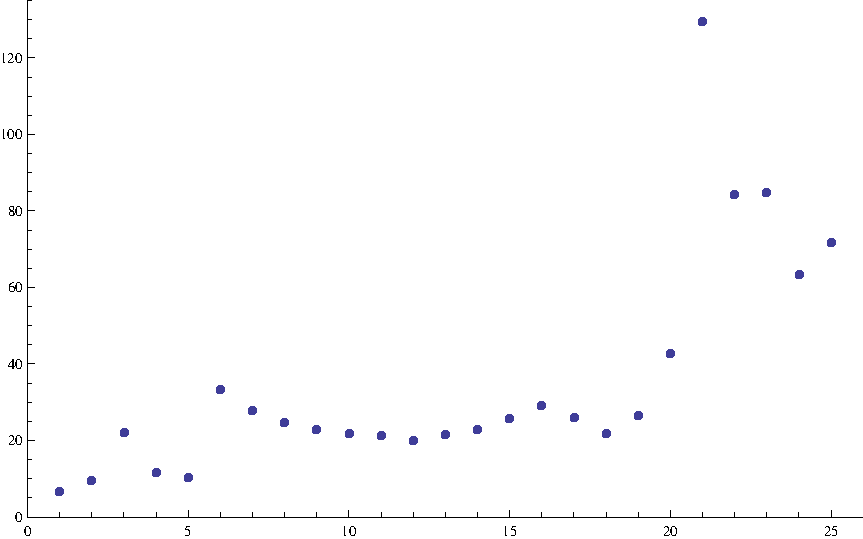
\includegraphics[width=\textwidth]{latencygraph.pdf}
    \caption{Latency in milliseconds over number of clients}
\end{figure}
\begin{figure}[h!]
    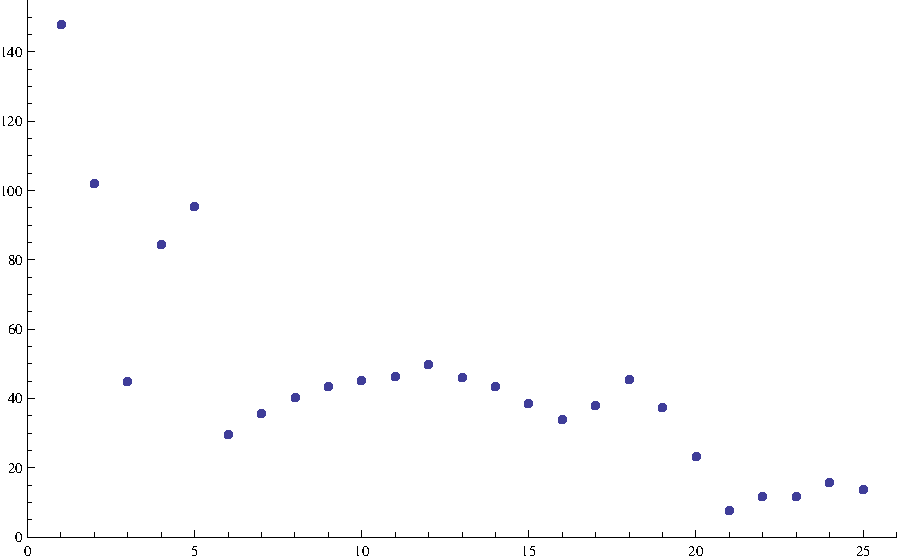
\includegraphics[width=\textwidth]{throughputgraph.pdf}
    \caption{Throughput in requests per second over number of clients}
\end{figure}

% Plot with latency over clients

\subsection{Question 7}
% Explain the effects you observe regarding throughput and latency of your service.
% Explain the plots..
The experiment shows the expected increase in latency, because of exclusive locking.
Therefore, the server will have to manage a lot of waiting requests, while
gaining no concurrency in calculation.

Since the throughput is just the inverse of the latency, a corresponding decrease
in throughput has been observed.


\subsection{Question 8}
% Given your response to Question 4, what other experiments would you use to quantify the
% performance of KeyValueBase? Justify your choices. (2 paragraphs) 
Since scans are item-concurrent, a comparison of scanning versus the other operations
will reveal the impact of bottlenecking at the index, and the possible gains from refining the
locking in other functions.

Measurement of throughput as a function of the element size. That is, small(4 bytes) to large(4MB)
values. This should show the overhead cost of a single insertion, with throughput increasing
linearly for larger values. If this is not the case, the scalability of the insertion method
is simply insufficient.


\subsection{Question 9}
{\tt atomicScan} is simply implemented by wrapping the {\tt Scan} function,
using the same lock as the other functions use.

{\tt bulkPut} is implemented by taking the lock at the start of insertion, as
well as locking the single elements (protection from scans), and releasing only
when the last value has been inserted.

\end{document}

